\chapter{Detection of dynamic gestures}

\section{Proposed methods}

The dynamic gesture recognition problem is a problem, where the input data consist of several consecutive positions and orientations of hand and fingers. 
Moreover, the important factor for recognition is the time dependencies between data frames. 
The slower and faster gestures should be recognized as the same dynamic gesture.

The proposed solution utilizes parts of the solution used for recognition of the static gestures.
Each frame of the captured data is described by the same features as in the static recognition part.
The set of features for each frame is then processed by the Hidden Markov Model scheme. 

\subsection{Hidden Markov Model}

Hidde Markov Model is a finite, $N$-element set of states, which are associated with the probability distribution.
The transitions between states are represented by the transition probabilities usually stored in $N\times N$ matrix $T$.
In every state, one of the observation from the finite, $K$-element observation set can be generated with observation probability usually represented by the $N\times K$ emission matrix $E$.
The finite set of all possible observation is called the alphabet.
To fully define the model, the definition of $N$-element vector of initial state probabilities $\Pi$.
Each HMM can be fully defined by the ($T$, $E$, $Pi$).

\begin{figure}[htb]
\centering
 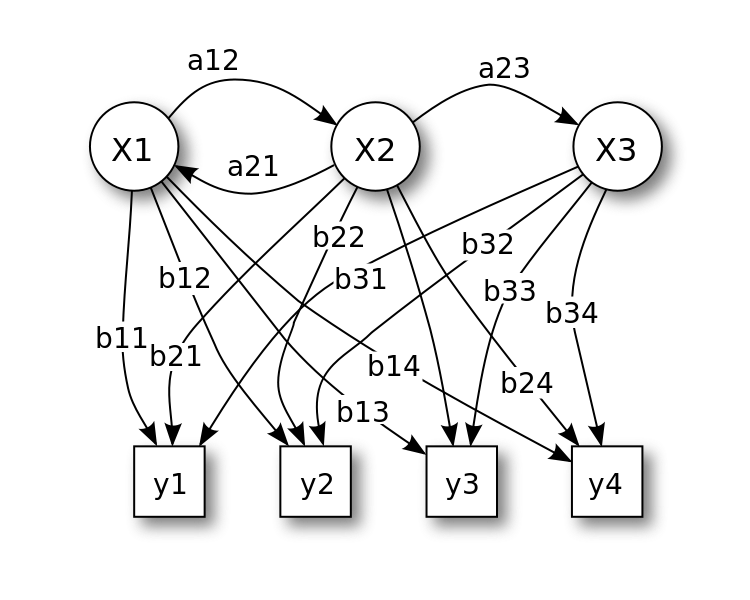
\includegraphics[width=0.8\columnwidth]{figures/HMM_wiki.png}
 \caption[]{Solution blocks of learning and testing parts in task of dynamic gesture recognition\footnotemark}
 \label{dynamicgestureswiki}
\end{figure}

\footnotetext{\url{http://en.wikipedia.org/wiki/File:HiddenMarkovModel.svg}}

The example HMM can be seen at fig.~\ref{dynamicgesturewiki}.
The HMM at the figure consists of 3 states ${X1, X2, X3}$ and 4 possible observations ${y1, y2, y3, y3}$.
The probabilities $a_{ij}$ define the transition probability from state $j$-th to state $i$-th. 
The probabilities $b_{ij}$ define the observation probability of generating $j$ observation while being in state $i$.

The HMM can be understood as a directed graph with two types of weighted vertices. 
This way, each state is represented by one type of vertices while observations can be shown as second type of vertices.
The edges between states contain and are an equivalent to the transition matrix. 
There are no edges between vertices representing observations.
The edges between states and observations are equal to the observation matrix.

$ xx $
There are three main algorithms used with the HMMs:
\begin{itemize}
\item Forward-Backward algorithm, 
\item Viterbi algorithm,
\item Baum-Welch algorithm.
\end{itemize}

The Forward-Backward algorithm is used to find the posterior probability of given states given the set of observations.
For the whole set of state variables $X = {X_i}_{i=1}^{N}$ and a set of observations $o_{1:t} = o_1, o_2,...,o_t$, the algorithm computes the $P(X_i | o_{1:t})$.
The algorithm utilizes a dynamic programming approach, by perfoming 3 steps in a loop: 
\begin{enumerate}
\item computing forward probabilities,
\item computing backward probabilites,
\item computing smoothed values.
\end{enumerate}
Firstly, the forward pass phase for $i=1,..,N$ computes the $P(X_i, o_{1:k})$, where $k$ is smaller than $t$, which represent the probability of ending up in state $X_i$ after first $k$ observations. 
The backward pass computes the $(P(o_{k+1:t}) | X_i)$, which are the probabilities of observing the rest of the observations in state $X_i$.
The smooting part, uses Bayes rule to compute the probability of state $X_i$ given the whole observation sequence:
\begin{equation}
P(X_k | o_{1:t}) = P(X_k | o_{1:k}, o_{k+1:t}) \propto P(o_{k+1:t} | X_k) P(X_k | o_{1:k})
\end{equation}
The time complexity of this algorithm is $O(N^2 T)$, where $T$ is the length of observation sequence and $N$ is the number of possible states.

The Viterbi algorithm is used to find the most likely sequence of hidden states that best explain the set of observations.
The set of those states is usually called the Viterbi path. 
Introduing the sequence:
\begin{equation}
V_{1,k} = P(o_1 | k) * \Pi_k)
\end{equation}
\begin{equation}
V_{t,k} = P(o_t | k) * argmax_{x\in X}(a_{x,k} * V_{t-1,x})
\end{equation}
Finally, the problem can be understood as finding the $argmax_{x\in X}(V_{T,x})$. 
The algorithm time complexity is the same as forward-backward $O(N^2 T)$.

The Baum-Welch algorithm is the algorithm used to find the unknown parameters of the HMM.
For each training example, the algorithms updates the state transition probabilities, observation probabilities in each state and intial probabilities to maximize the likelihood of observation.
Having the set of sets of observations, the algorithm can be used to train HMM to detect the sequences similiar to the ones used in learning process.

\begin{figure}[htb]
\centering
 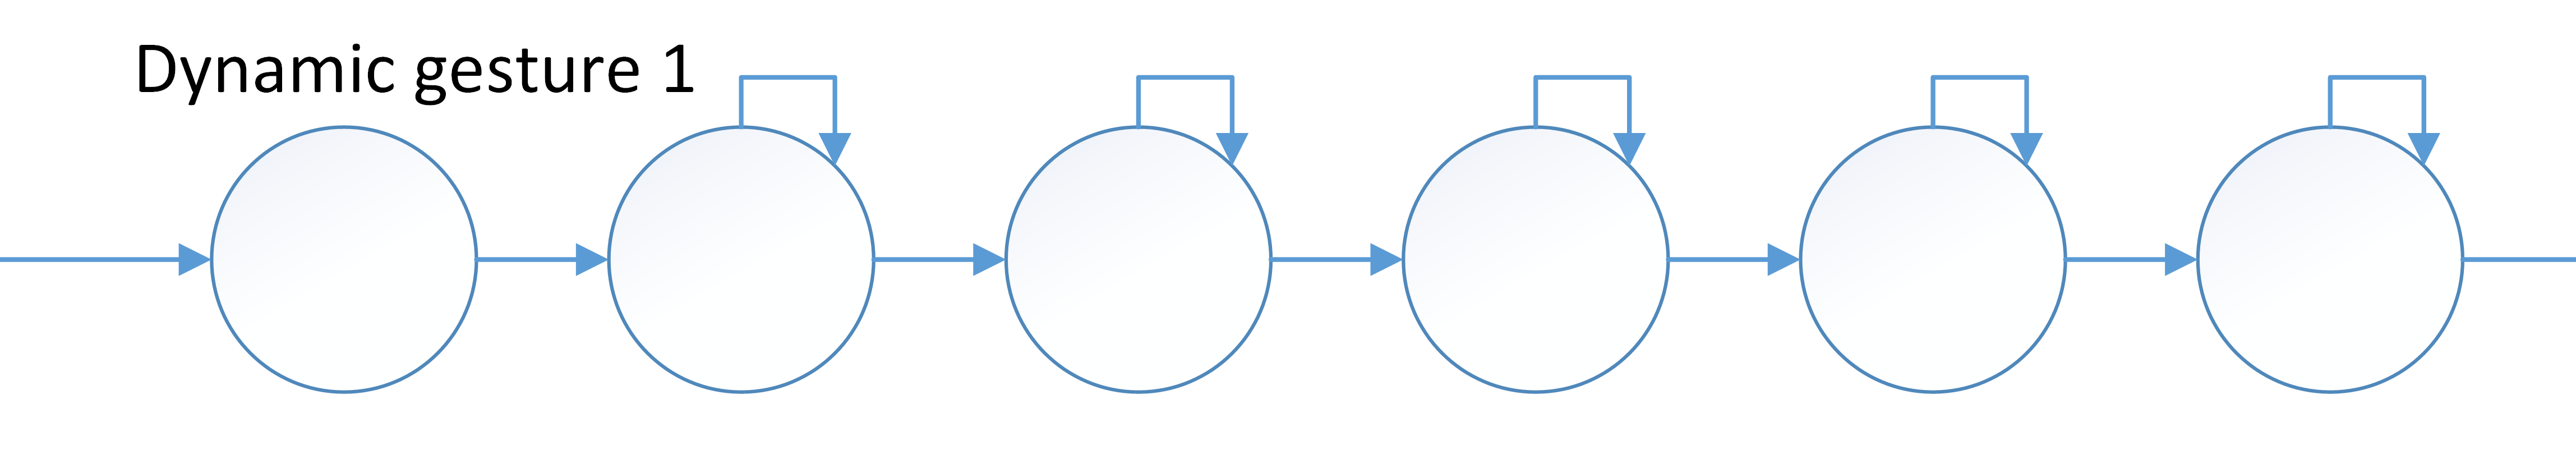
\includegraphics[width=1\columnwidth]{figures/SingleHMM.png}
 \caption{Non-zero state transitions and states of the HMM used to detect single dynamic gesture}
 \label{singlehmm}
\end{figure}

In the dynamic gesture recognition task, we adopted a structure of HMM with state having non-zero transition probabilites to self and to the next state in the sequence.
The proposed structe is presented at fig.~\ref{singlehmm} 
The states can be understood as the phases of hand movement and position that happen when the wanted gesture is performed.
The self-transitions are used to model the different speeds of the gestures.
This structure after training process can be used to measure the probability of that the dynamic gesture occured given the set of observations.

\begin{figure}[htb]
\centering
 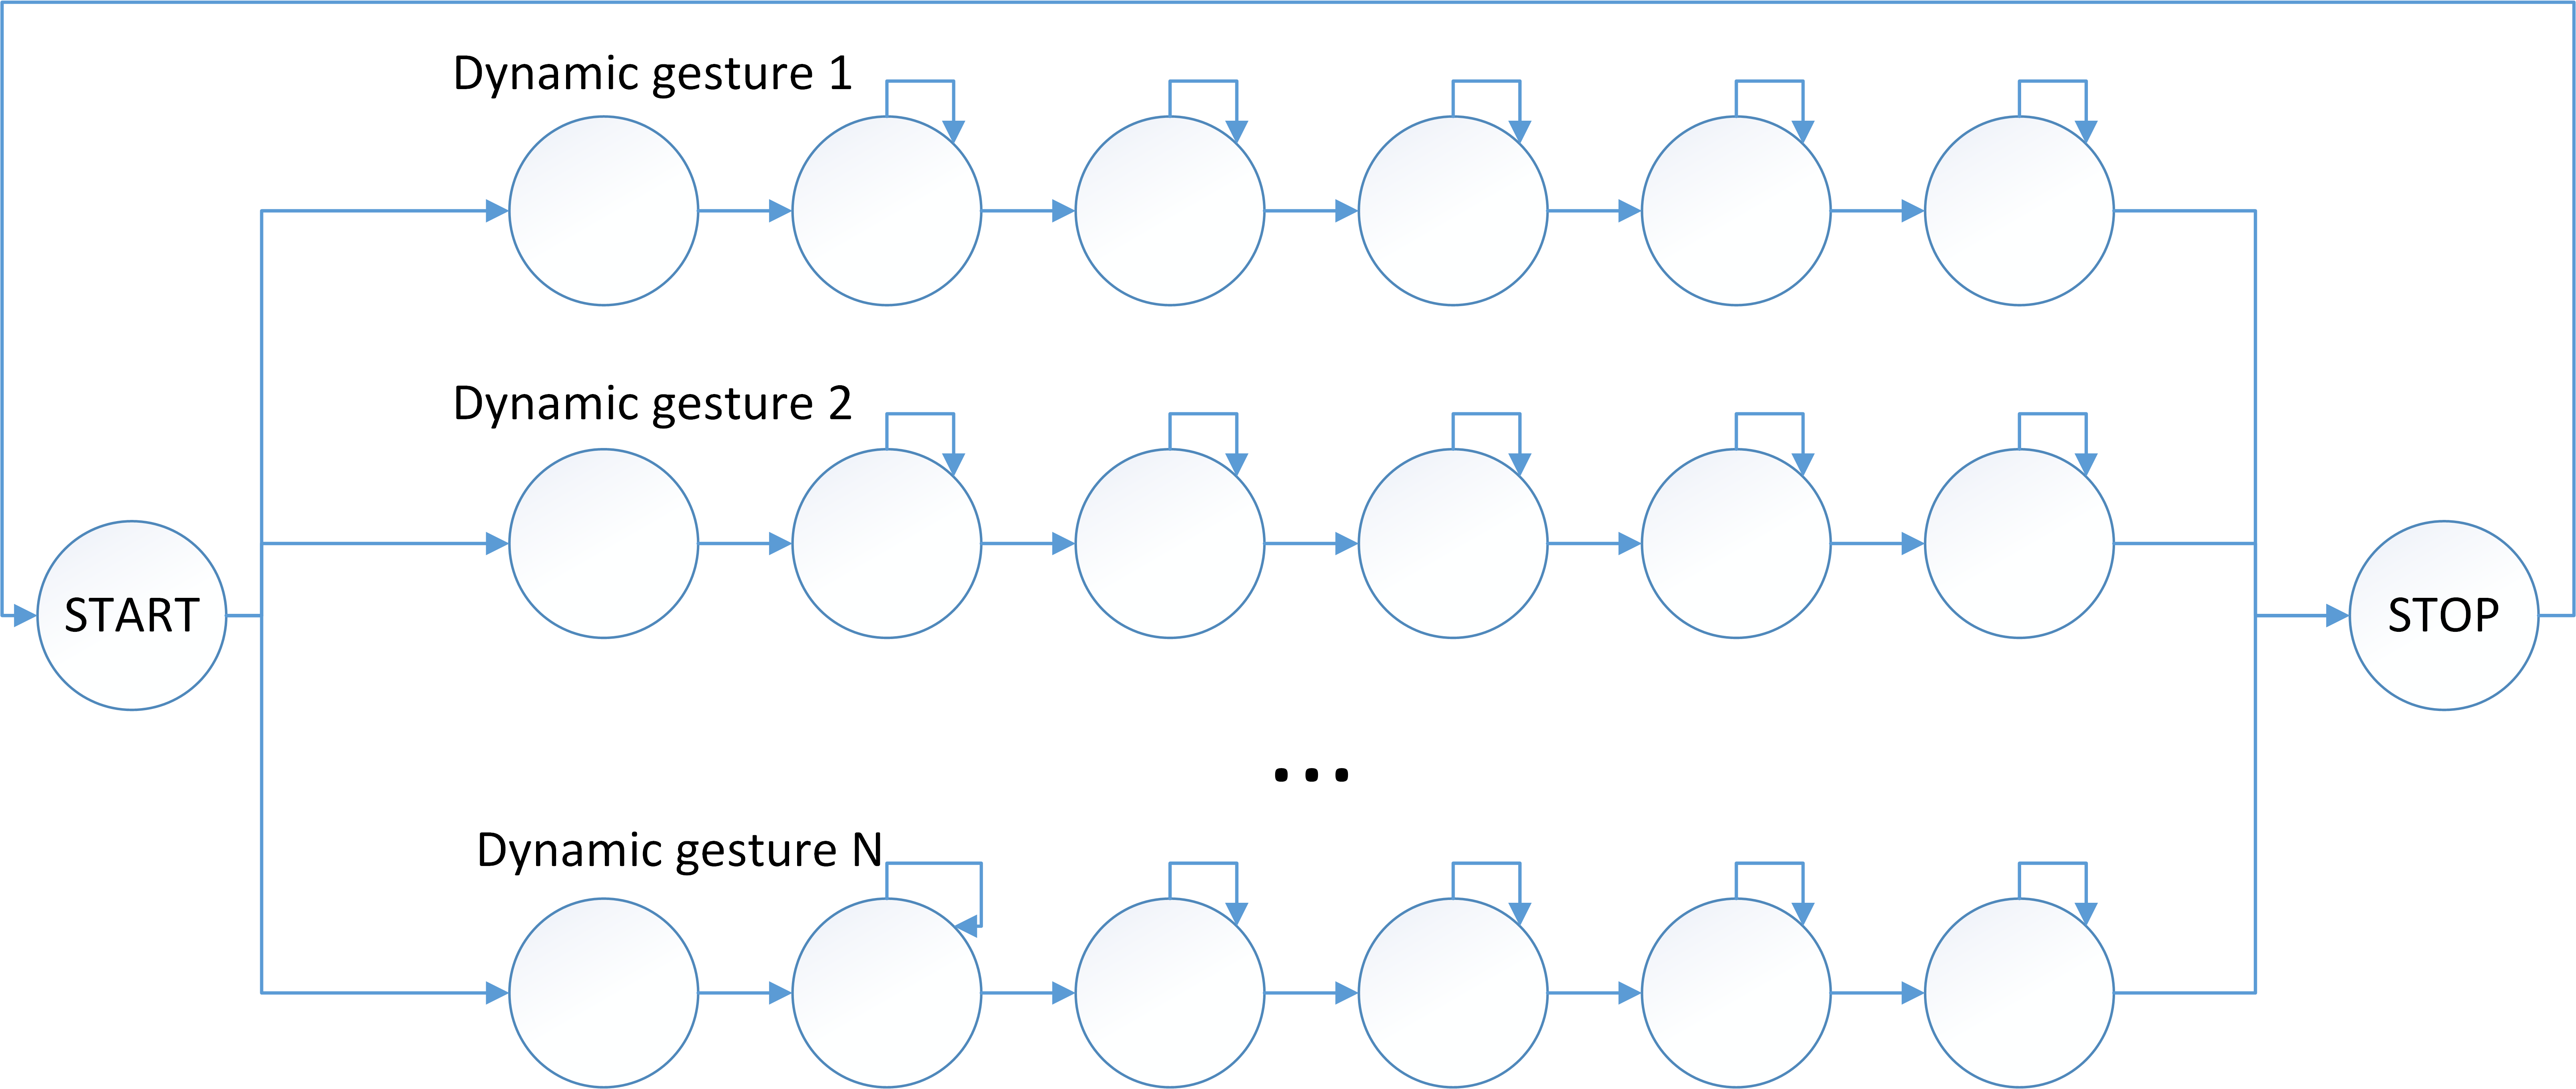
\includegraphics[width=1\columnwidth]{figures/HMM_eng.png}
 \caption{Non-zero state transitions and states for the HMM enabling simulatneous detection of $m$ dynamic gestures}
 \label{HMMstructure}
\end{figure}

Having single dynamic gesture recognition problem modelled as the sequence of $n$ states in which $kths$ state is connected by the edges to the $k$ and $(k+1)$ state and to the all observations.
Having the problem of distinguishing $m$ gestures translates to the $m$ sequential graphs.
The problem of finding if and what dyanmic gesture occured is the problem of finding the probabilities from each $m$ HMM and checking them against preset threshold.
Alternatively, the $m$ HMMs can be combined into one HMM were those single HMMs are treated as parallel paths.
The structure of proposed single HMM is presented at fig.~\ref{HMMstructure}.
Then the recognitnion process is a process of finding, which of the parallel paths is the most probable.
The only remaining problem is the problem of preparing the set of ccured, 1-dimensional observations from the Leap Motion data.

\subsection{HMM observation from Leap Motion data}

Most of the proposed solutions in the literature assume that the observations are 1-dimensional.
There were attempts to expand the HMM to the 2-dimensional observations [], but the raw data from Leap Motion is defined in higer-dimensional that any found solution.
That is the reason, why the need to reduce the dimensionality of the observation of the single hand in the predefined moment in time.

To do this, unsupervised clustering algorithms were used.

***********************
**************8
Opisać algorytmy
Opisać metody doboru liczby klas
********


\begin{figure}[htb]
\centering
 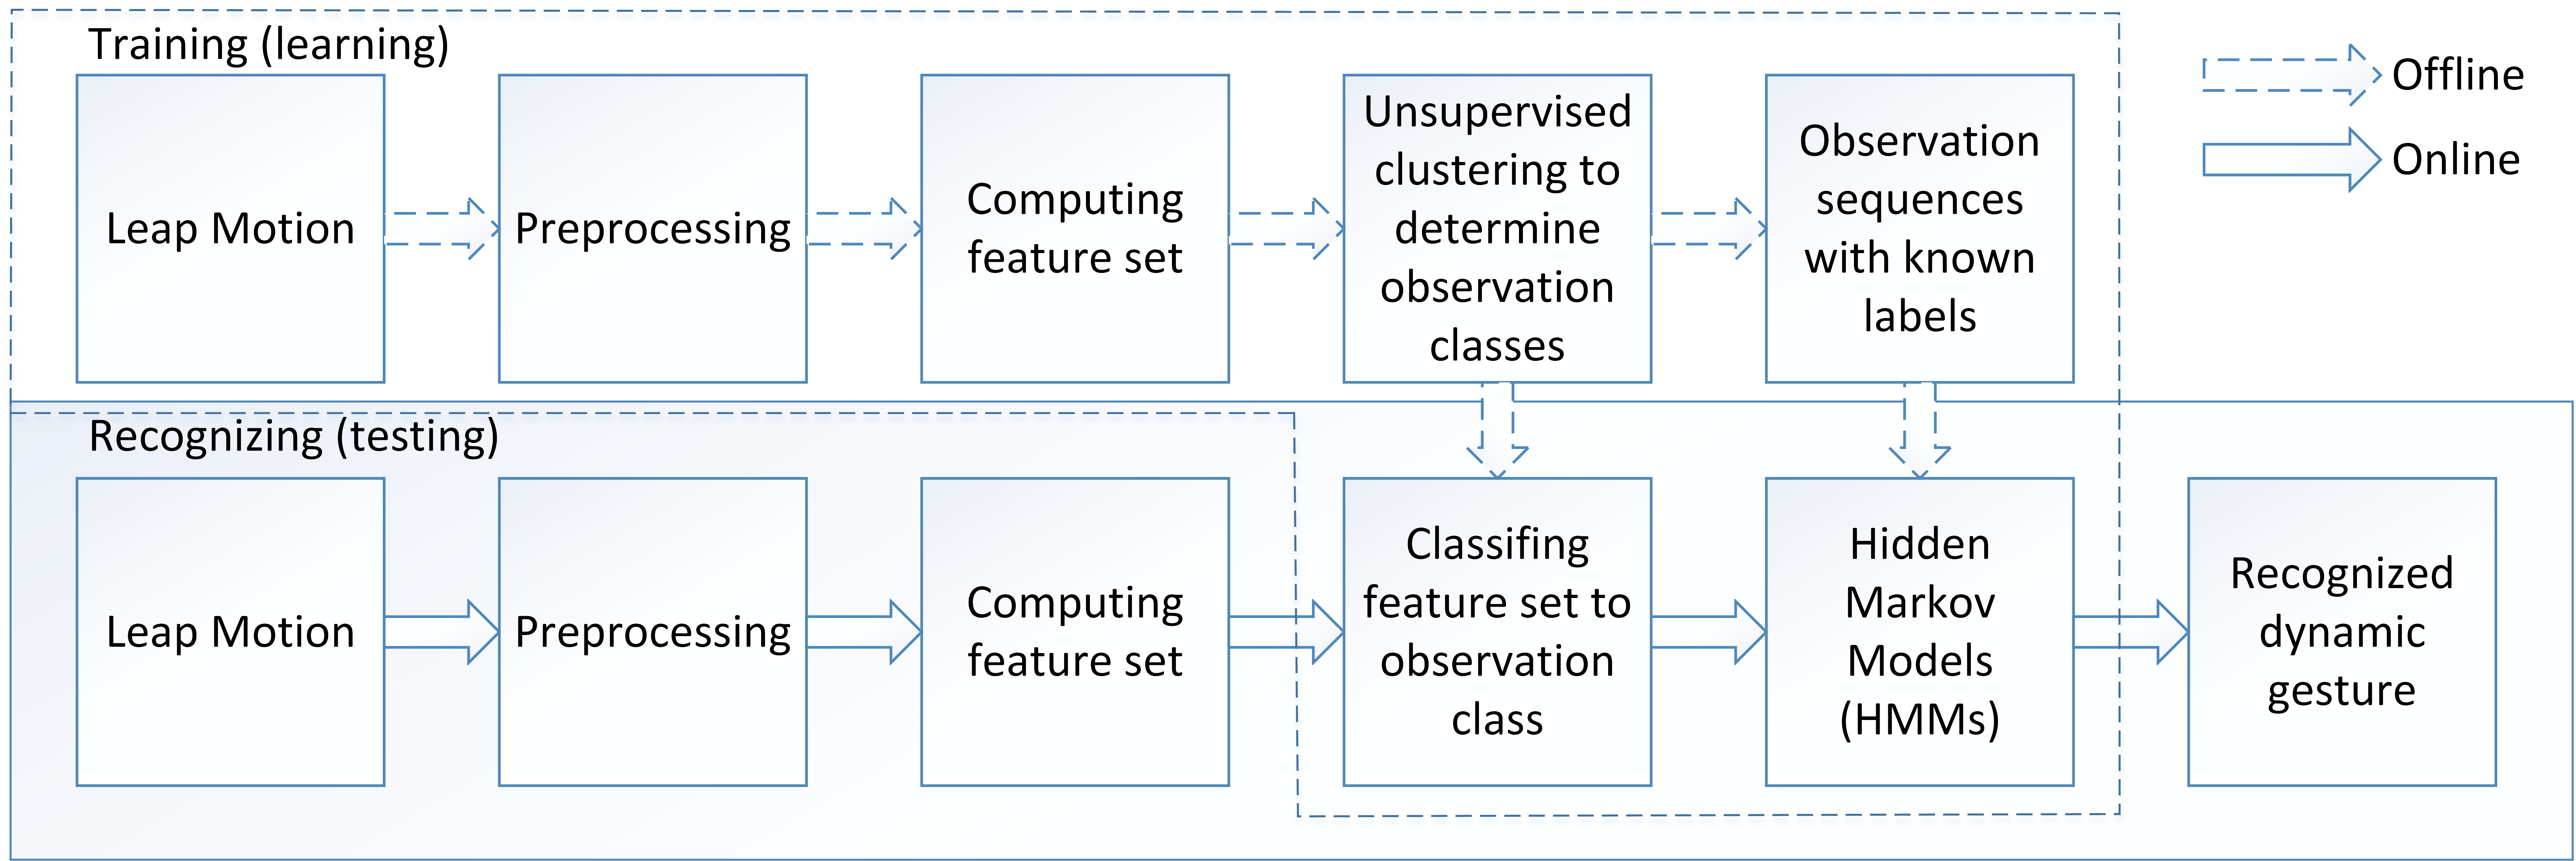
\includegraphics[width=1\columnwidth]{figures/DynamicGestures.png}
 \caption{Solution blocks of learning and testing parts in task of dynamic gesture recognition}
 \label{dynamicgesturesflow}
\end{figure}

Finally, the whole processing flow has been desgined and is presented at fig.~\ref{dynamicgesturesflow}.
The whole solution consists of two parts: offline learning and online recognition.
For learning, the raw data is preprocessed and then the feature are extracted. 
Similarly to the static gestures, the features set containing the finger count, angles between fingers and normal of hand, angles between fingers and distances between finger's tips were used. 
In traning part, those features are extracted from all recorded positions for all dynamic gestures.
Then one of the unsupervised clustering algorithms is used to find the classes of observations (usually 8-12 classes worked best).
Knowledge of the classes is used to represent each dynamic gesture as a series of one-dimensional observations.
After that for each dynamic gesture, the corresponding HMM is learned by running the Baum-Welch algorithm on the sequence of observations.
To complete, the training process, the HMMs are combined into one HMM.

In the online working, the raw data from leap motion is preprocessed, then each frame is labeled accordingly to the classes learnt by the unsupervised clustering algorithm.
The next step include providing the set of observations to HMM and running the Viterbi algorithm.
The Viterbi algorithm finds the most likely sequence in one the parallel paths, which informs us about the number of the found gesture. 
If the likelihood is above preset threshold, the gesture is assumed to be correctly recognized.


\section{Evaluation methodology}

To evaluate proposed approach ... 






  






The proposed solution utilizes Hidden Markov Model[] 



\section{Experiments}
